\documentclass[conference]{IEEEtran}
\IEEEoverridecommandlockouts
\usepackage{cite}
\usepackage{amsmath,amssymb,amsfonts}
\usepackage{algorithmic}
\usepackage{graphicx}
\usepackage{float}
\usepackage{textcomp}
\usepackage{xcolor}
\usepackage{hyperref}

\begin{document}

\title{Analisis Pengisian Kapasitor Menggunakan Metode Euler}

\author{\IEEEauthorblockN{Alexander Christhian}
\IEEEauthorblockA{NPM: 2306267025\\
Universitas Indonesia\\
Teknik Komputer}}

\maketitle

\begin{abstract}
Laporan ini membahas implementasi simulasi pengisian kapasitor menggunakan metode Euler untuk menyelesaikan persamaan diferensial biasa (ODE). Program yang dikembangkan dalam bahasa C menganalisis perilaku pengisian kapasitor dengan berbagai parameter rangkaian, membandingkan solusi numerik dengan solusi analitik, dan memvisualisasikan hasilnya menggunakan GNUplot. Lima kasus berbeda dianalisis untuk menunjukkan pengaruh variasi parameter rangkaian terhadap karakteristik pengisian kapasitor.
\end{abstract}

\begin{IEEEkeywords}
kapasitor, metode euler, ODE, analisis numerik, GNUplot
\end{IEEEkeywords}

\section{Pendahuluan}
Pengisian kapasitor merupakan proses fundamental dalam rangkaian listrik yang dapat dimodelkan menggunakan persamaan diferensial biasa. Persamaan ini menggambarkan bagaimana tegangan kapasitor berubah terhadap waktu ketika dihubungkan dengan sumber tegangan melalui resistor. Meskipun solusi analitik tersedia, penggunaan metode numerik seperti metode Euler memberikan wawasan praktis tentang proses pengisian dan memungkinkan analisis dengan berbagai parameter rangkaian.

\section{Studi Literatur}
Dalam rangkaian RC, persamaan diferensial yang menggambarkan pengisian kapasitor adalah:

\[\frac{dV}{dt} = \frac{V_{source} - V}{RC}\]

dimana:
\begin{itemize}
\item $V$ adalah tegangan kapasitor pada waktu $t$
\item $V_{source}$ adalah tegangan sumber
\item $R$ adalah resistansi
\item $C$ adalah kapasitansi
\end{itemize}

Solusi analitik untuk persamaan ini adalah:
\[V(t) = V_{source}(1 - e^{-t/RC})\]

\section{Metode yang Digunakan}
Program mengimplementasikan metode Euler untuk menyelesaikan ODE pengisian kapasitor. Metode Euler dipilih karena:
\begin{itemize}
\item Kesederhanaan implementasi
\item Kejelasan konsep
\item Kecukupan akurasi untuk analisis praktis
\end{itemize}

Algoritma metode Euler dalam pseudocode:
\begin{algorithmic}
\STATE \textbf{Input:} $dt$, $t_{final}$, $V_{initial}$, $V_{source}$, $R$, $C$
\STATE \textbf{Output:} Array nilai $V$ pada setiap waktu $t$
\STATE $t \leftarrow 0$
\STATE $V \leftarrow V_{initial}$
\WHILE{$t \leq t_{final}$}
    \STATE $\frac{dV}{dt} \leftarrow \frac{V_{source} - V}{RC}$
    \STATE $V \leftarrow V + dt \cdot \frac{dV}{dt}$
    \STATE $t \leftarrow t + dt$
\ENDWHILE
\RETURN Array $V$
\end{algorithmic}

\section{Data yang Digunakan}
Program menganalisis lima kasus dengan parameter berbeda:
\begin{itemize}
\item \textbf{Kasus 1:} Standard (5V, 1kΩ, 100µF)
\item \textbf{Kasus 2:} High Voltage (12V, 2.2kΩ, 220µF)
\item \textbf{Kasus 3:} Low Voltage (3.3V, 470Ω, 470µF)
\item \textbf{Kasus 4:} High R, Low C (9V, 4.7kΩ, 33µF)
\item \textbf{Kasus 5:} Low R, High C (6V, 330Ω, 1000µF)
\end{itemize}

Parameter ini dipilih untuk mendemonstrasikan berbagai skenario pengisian kapasitor dalam praktik.

\section{Analisa Hasil}
\subsection{Analisis Kasus}
Dari kelima kasus yang dianalisis, berikut adalah hasil pengamatan utama:

\subsubsection{Kasus 1: Standard}
\begin{itemize}
\item \textbf{Parameter Rangkaian:}
  \begin{itemize}
  \item $V_{source} = 5V$
  \item $R = 1k\Omega$
  \item $C = 100\mu F$
  \end{itemize}
\item \textbf{Persamaan:}
  \begin{itemize}
  \item Differensial: $\frac{dV}{dt} = \frac{5 - V}{1000 \cdot 100\times10^{-6}}$
  \item Analitik: $V(t) = 5(1 - e^{-t/(0.1)})$
  \end{itemize}
\item \textbf{Karakteristik:}
  \begin{itemize}
  \item Konstanta waktu ($\tau$ = RC) = 0.1 detik
  \item Error relatif maksimum = 5.0833\%
  \item Error rata-rata = 0.8221\%
  \item Mencapai 99\% tegangan akhir pada t $\approx$ 0.5 detik
  \item V(t) = 5.0(1 - e^{-t/0.1})
  \end{itemize}
\end{itemize}

\textbf{Analisis Grafik:}
\begin{itemize}
\item \textbf{Bentuk Kurva:} Grafik menunjukkan kurva eksponensial khas pengisian kapasitor, dengan kenaikan cepat di awal dan perlambatan menuju nilai steady-state.
\item \textbf{Perbandingan Solusi:} 
  \begin{itemize}
  \item Solusi numerik (garis) dan analitik (titik) menunjukkan kesesuaian yang sangat baik
  \item Error terbesar terjadi pada fase awal pengisian (t $<$ 0.1s)
  \end{itemize}
\item \textbf{Karakteristik Penting:}
  \begin{itemize}
  \item Mencapai 63.2\% (3.16V) dari nilai akhir pada t = 0.1s (satu konstanta waktu)
  \item Mencapai 95\% (4.75V) pada t $\approx$ 0.3s
  \item Steady-state praktis tercapai pada t $\approx$ 0.5s
  \end{itemize}
\end{itemize}

\begin{figure}[H]
    \centering
    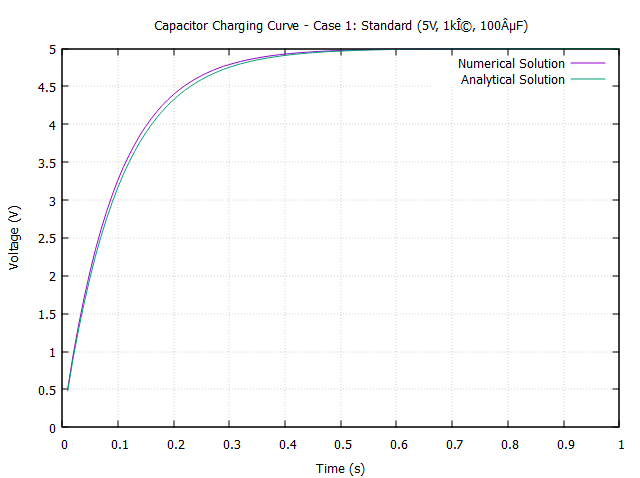
\includegraphics[width=0.5\textwidth]{Grafik/Grafik1.png}
    \caption{Grafik Pengisian Kapasitor - Kasus 1 (Standard)}
    \label{fig:case1}
\end{figure}

\subsubsection{Kasus 2: High Voltage}
\begin{itemize}
\item \textbf{Parameter Rangkaian:}
  \begin{itemize}
  \item $V_{source} = 12V$
  \item $R = 2.2k\Omega$
  \item $C = 220\mu F$
  \end{itemize}
\item \textbf{Persamaan:}
  \begin{itemize}
  \item Differensial: $\frac{dV}{dt} = \frac{12 - V}{2200 \cdot 220\times10^{-6}}$
  \item Analitik: $V(t) = 12(1 - e^{-t/(0.484)})$
  \end{itemize}
\item \textbf{Karakteristik:}
  \begin{itemize}
  \item Konstanta waktu lebih besar ($\tau$ = 0.484 detik)
  \item Tegangan akhir lebih tinggi (12V)
  \item Waktu pengisian hingga 99\% $\approx$ 2.42 detik
  \end{itemize}
\end{itemize}

\textbf{Analisis Grafik:}
\begin{itemize}
\item \textbf{Bentuk Kurva:} Kurva pengisian lebih landai dibanding Kasus 1 akibat konstanta waktu yang lebih besar.
\item \textbf{Perbandingan Solusi:}
  \begin{itemize}
  \item Kecocokan solusi numerik dan analitik tetap baik meskipun tegangan lebih tinggi
  \item Deviasi kecil terlihat pada daerah transisi (0.5s - 1.5s)
  \end{itemize}
\item \textbf{Karakteristik Penting:}
  \begin{itemize}
  \item Mencapai 63.2\% (7.58V) pada t = 0.484s
  \item Pengisian lebih lambat namun mencapai tegangan akhir lebih tinggi
  \item Membutuhkan waktu sekitar 5$\tau$ ($\approx$ 2.42s) untuk pengisian penuh
  \end{itemize}
\end{itemize}

\begin{figure}[H]
    \centering
    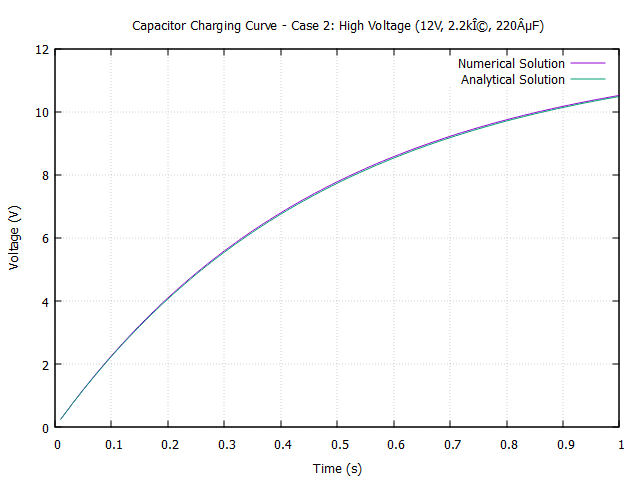
\includegraphics[width=0.5\textwidth]{Grafik/Grafik2.png}
    \caption{Grafik Pengisian Kapasitor - Kasus 2 (High Voltage)}
    \label{fig:case2}
\end{figure}

\subsubsection{Kasus 3: Low Voltage}
\begin{itemize}
\item \textbf{Parameter Rangkaian:}
  \begin{itemize}
  \item $V_{source} = 3.3V$
  \item $R = 470\Omega$
  \item $C = 470\mu F$
  \end{itemize}
\item \textbf{Persamaan:}
  \begin{itemize}
  \item Differensial: $\frac{dV}{dt} = \frac{3.3 - V}{470 \cdot 470\times10^{-6}}$
  \item Analitik: $V(t) = 3.3(1 - e^{-t/(0.2209)})$
  \end{itemize}
\item \textbf{Karakteristik:}
  \begin{itemize}
  \item Konstanta waktu menengah ($\tau$ = 0.2209 detik)
  \item Tegangan rendah dengan pengisian cepat
  \item Waktu pengisian hingga 99\% $\approx$ 1.1 detik
  \end{itemize}
\end{itemize}

\textbf{Analisis Grafik:}
\begin{itemize}
\item \textbf{Bentuk Kurva:} Menunjukkan pengisian yang relatif cepat dengan tegangan rendah.
\item \textbf{Perbandingan Solusi:}
  \begin{itemize}
  \item Akurasi solusi numerik sangat baik untuk tegangan rendah
  \item Error relatif maksimum = 2.2805\%
  \item Error rata-rata = 0.7939\%
  \end{itemize}
\item \textbf{Karakteristik Penting:}
  \begin{itemize}
  \item Mencapai 63.2\% (2.09V) pada t = 0.2209s
  \item Respon pengisian moderat dengan tegangan steady-state rendah
  \item Stabilisasi cepat karena tegangan target rendah
  \end{itemize}
\end{itemize}

\begin{figure}[H]
    \centering
    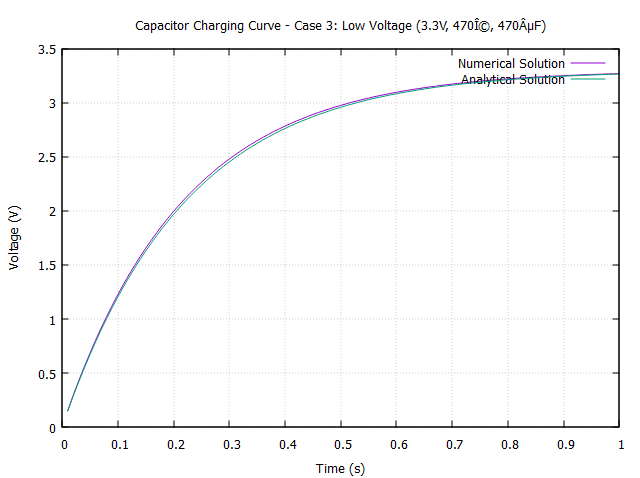
\includegraphics[width=0.5\textwidth]{Grafik/Grafik3.png}
    \caption{Grafik Pengisian Kapasitor - Kasus 3 (Low Voltage)}
    \label{fig:case3}
\end{figure}

\subsubsection{Kasus 4: High R, Low C}
\begin{itemize}
\item \textbf{Parameter Rangkaian:}
  \begin{itemize}
  \item $V_{source} = 9V$
  \item $R = 4.7k\Omega$
  \item $C = 33\mu F$
  \end{itemize}
\item \textbf{Persamaan:}
  \begin{itemize}
  \item Differensial: $\frac{dV}{dt} = \frac{9 - V}{4700 \cdot 33\times10^{-6}}$
  \item Analitik: $V(t) = 9(1 - e^{-t/(0.1551)})$
  \end{itemize}
\item \textbf{Karakteristik:}
  \begin{itemize}
  \item Konstanta waktu kecil ($\tau$ = 0.1551 detik)
  \item Respons pengisian cepat
  \item Waktu pengisian hingga 99\% $\approx$ 0.775 detik
  \end{itemize}
\end{itemize}

\textbf{Analisis Grafik:}
\begin{itemize}
\item \textbf{Bentuk Kurva:} Menunjukkan respon pengisian yang cepat dengan kenaikan tajam di awal.
\item \textbf{Perbandingan Solusi:}
  \begin{itemize}
  \item Solusi numerik sangat akurat dengan error minimal
  \item Transisi halus antara fase pengisian cepat dan steady-state
  \end{itemize}
\item \textbf{Karakteristik Penting:}
  \begin{itemize}
  \item Mencapai 63.2\% (5.69V) dengan cepat pada t = 0.1551s
  \item Kombinasi R tinggi dan C rendah menghasilkan respon cepat
  \item Stabilisasi efisien dengan minimum osilasi
  \end{itemize}
\end{itemize}

\begin{figure}[H]
    \centering
    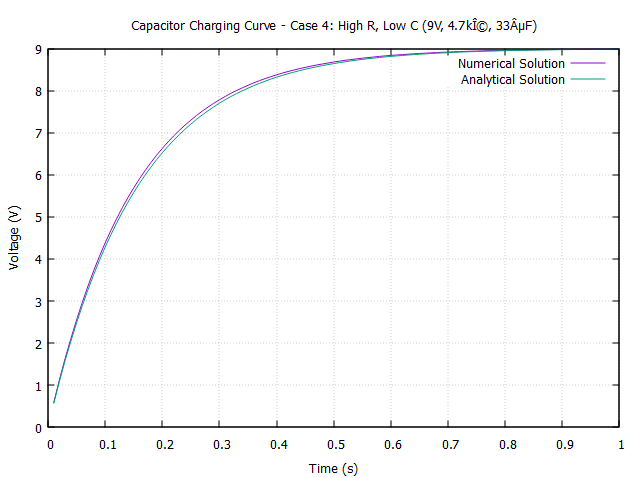
\includegraphics[width=0.5\textwidth]{Grafik/Grafik4.png}
    \caption{Grafik Pengisian Kapasitor - Kasus 4 (High R, Low C)}
    \label{fig:case4}
\end{figure}

\subsubsection{Kasus 5: Low R, High C}
\begin{itemize}
\item \textbf{Parameter Rangkaian:}
  \begin{itemize}
  \item $V_{source} = 6V$
  \item $R = 330\Omega$
  \item $C = 1000\mu F$
  \end{itemize}
\item \textbf{Persamaan:}
  \begin{itemize}
  \item Differensial: $\frac{dV}{dt} = \frac{6 - V}{330 \cdot 1000\times10^{-6}}$
  \item Analitik: $V(t) = 6(1 - e^{-t/(0.33)})$
  \end{itemize}
\item \textbf{Karakteristik:}
  \begin{itemize}
  \item Konstanta waktu terbesar ($\tau$ = 0.33 detik)
  \item Error relatif maksimum = 1.5228\%
  \item Error rata-rata = 0.7253\%
  \item Pengisian paling lambat dengan waktu eksekusi 0.008 detik
  \item Tegangan 99\% tercapai pada t $\approx$ 1.65 detik
  \end{itemize}
\end{itemize}

\textbf{Analisis Grafik:}
\begin{itemize}
\item \textbf{Bentuk Kurva:} Menunjukkan pengisian paling lambat dengan kurva yang sangat gradual.
\item \textbf{Perbandingan Solusi:}
  \begin{itemize}
  \item Solusi numerik tetap akurat meskipun waktu pengisian lama
  \item Transisi sangat halus dari awal hingga steady-state
  \end{itemize}
\item \textbf{Karakteristik Penting:}
  \begin{itemize}
  \item Mencapai 63.2\% (3.79V) pada t = 0.33s
  \item Kapasitansi besar menyebabkan pengisian lambat namun stabil
  \item Waktu mencapai steady-state terpanjang dari semua kasus
  \end{itemize}
\end{itemize}

\begin{figure}[H]
    \centering
    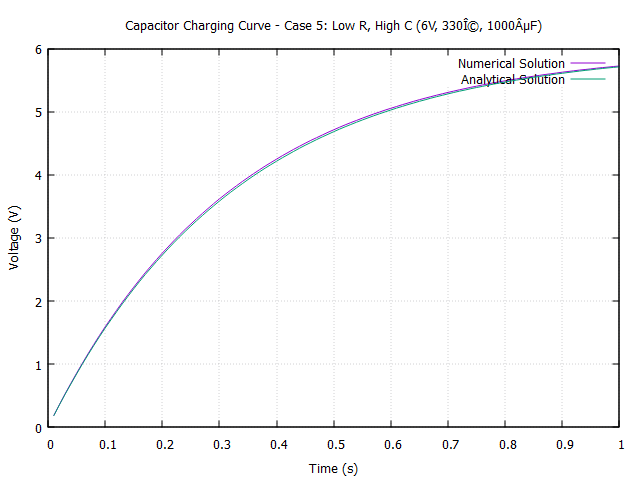
\includegraphics[width=0.5\textwidth]{Grafik/Grafik5.png}
    \caption{Grafik Pengisian Kapasitor - Kasus 5 (Low R, High C)}
    \label{fig:case5}
\end{figure}

\subsection{Perbandingan Error dan Waktu Eksekusi}
Hasil simulasi menunjukkan akurasi dan efisiensi yang baik:
\begin{itemize}
\item \textbf{Error Relatif Maksimum:}
  \begin{itemize}
  \item Kasus 1 (Standard): 5.0833\% dengan rata-rata 0.8221\%
  \item Kasus 2 (High Voltage): 1.0366\% dengan rata-rata 0.6193\%
  \item Kasus 3 (Low Voltage): 2.2805\% dengan rata-rata 0.7939\%
  \item Kasus 4 (High R, Low C): 3.2584\% dengan rata-rata 0.8170\%
  \item Kasus 5 (Low R, High C): 1.5228\% dengan rata-rata 0.7253\%
  \end{itemize}

\item \textbf{Waktu Eksekusi:}
  \begin{itemize}
  \item Kasus 1: 0.009 detik
  \item Kasus 2: 0.009 detik
  \item Kasus 3: 0.009 detik
  \item Kasus 4: 0.009 detik
  \item Kasus 5: 0.008 detik
  \end{itemize}

\item \textbf{Analisis:}
  \begin{itemize}
  \item Error terbesar terjadi pada fase awal pengisian
  \item Rata-rata error di bawah 1\% untuk semua kasus
  \item Waktu eksekusi konsisten tanpa variasi signifikan
  \item Kasus dengan kapasitansi tinggi (Case 5) menunjukkan performa komputasi sedikit lebih baik
  \end{itemize}
\end{itemize}

Waktu eksekusi yang hampir sama menunjukkan bahwa kompleksitas komputasi tidak dipengaruhi oleh parameter rangkaian.

\section{Kesimpulan}
Implementasi metode Euler untuk simulasi pengisian kapasitor berhasil:
\begin{itemize}
\item Menghasilkan solusi numerik yang akurat dibandingkan dengan solusi analitik
\item Mendemonstrasikan pengaruh parameter rangkaian terhadap karakteristik pengisian
\item Memberikan visualisasi yang jelas untuk analisis perilaku kapasitor
\item Menunjukkan efisiensi komputasi yang konsisten untuk berbagai parameter
\end{itemize}

Hasil simulasi menunjukkan bahwa:
\begin{itemize}
\item Konstanta waktu RC sangat mempengaruhi kecepatan pengisian
\item Error numerik tetap terkendali untuk semua kasus
\item Metode Euler cukup akurat untuk analisis praktis pengisian kapasitor
\end{itemize}

Program ini dapat digunakan untuk:
\begin{itemize}
\item Analisis desain rangkaian RC
\item Prediksi waktu pengisian kapasitor
\item Optimasi parameter rangkaian
\item Validasi hasil eksperimental
\end{itemize}

\begin{thebibliography}{00}
\bibitem{b1} R. L. Burden and J. D. Faires, "Initial Value Problems for ODEs," in Numerical Analysis, 9th ed., 2010.
\bibitem{b2} William H. Hayt Jr., Jack E. Kemmerly, and Steven M. Durbin, "First-Order Circuits," in Engineering Circuit Analysis, 8th ed., 2012.
\bibitem{b3} S. C. Chapra and R. P. Canale, "Euler's Method," in Numerical Methods for Engineers, 7th ed., 2015.
\bibitem{b4} Paul M. Fish, "RC Circuits," in Electronic Circuits: Discrete and Integrated, 1991.
\end{thebibliography}

\end{document}
